% Chinese narrative; English equations/descriptions, tables, and figure captions.
\documentclass[journal]{IEEEtran}
\usepackage[UTF8,fontset=none,scheme=plain]{ctex}
\setmainfont{TeX Gyre Termes}
\setCJKmainfont{Noto Serif CJK SC}
\setCJKsansfont{Noto Sans CJK SC}
\setCJKmonofont{Noto Sans Mono CJK SC}
\usepackage{amsmath,amssymb,booktabs,array,graphicx,tabularx}
\usepackage{placeins,xurl}
\usepackage[hidelinks,unicode,breaklinks=true]{hyperref}
\urlstyle{same}
\renewcommand{\abstractname}{摘要}
\renewcommand{\IEEEkeywordsname}{关键词}
\renewcommand{\refname}{参考文献}
\newcolumntype{L}[1]{>{\raggedright\arraybackslash}p{#1}}
\newcolumntype{C}{>{\centering\arraybackslash}X}
% Align and group floats at the top of float-only pages.
\makeatletter
\setlength{\@fptop}{0pt}
\setlength{\@fpsep}{12pt}
\setlength{\@dblfptop}{0pt}
\setlength{\@dblfpsep}{12pt}
\makeatother
\title{ReCA-SAM3: RemoteCLIP-Guided Cross-Class Feature Aggregation for Open-Vocabulary Remote Sensing Semantic Segmentation}
\author{}
\begin{document}
\maketitle
\begin{abstract}
开放词汇遥感语义分割需要在复杂空间布局中识别文本指定的地物类别。图文匹配提供领域语义，概念分割模型提供空间表征，如何将二者用于解码前的类别交互仍有待研究。本文提出 ReCA-SAM3，将 RemoteCLIP 的模板级图文相似度与最终稠密图像特征编码为类别相关的语义引导。该引导在聚合过程中保持不变，与 SAM 3 类别条件特征共同构造注意力的查询和键，值由条件特征提供。每个聚合块先进行类间特征交互，再以共享权重的三尺度普通窗口注意力建模提示内部的空间联系；各尺度更新对齐后经可学习权重融合，仅残差更新 SAM 3 条件特征。语义—细节融合模块进一步结合聚合特征、原始条件特征和图像空间特征，接入冻结的 SAM 3 解码器。训练结合分割监督与原始 SAM 3 软掩码蒸馏，为领域适配提供预测约束。
\end{abstract}

\begin{IEEEkeywords}
开放词汇语义分割，遥感，SAM 3，RemoteCLIP，跨类别特征聚合。
\end{IEEEkeywords}
\section{引言}
开放词汇语义分割通过类别文本指定待识别对象，为遥感图像中多样化地物的解译提供了灵活接口。遥感场景具有显著的尺度差异、任意方向分布和复杂空间布局；草地与耕地等地物还可能呈现相近的局部纹理。像素级预测既需要可靠的语义判别，也需要维持区域结构和细节。如何在跨场景使用文本类别时协调这两类需求，是开放词汇遥感分割的重要问题。

CLIP 的图文表征为开放词汇识别提供了基础~\cite{radfordLearningTransferableVisual2021}。RemoteCLIP 通过遥感图文预训练引入领域知识~\cite{liuRemoteCLIPVisionLanguage2024}，GSNet 将通用与遥感专用视觉特征融合，并通过专门的解码模块恢复细节~\cite{yeOpenVocabularyRemoteSensing2025}。CAT-Seg 将局部图文相似度编码为代价表征，再进行空间与类别聚合~\cite{choCATSegCostAggregation2024}；RSKT-Seg 将这一方向扩展到遥感，结合多方向匹配、代价融合及领域知识迁移~\cite{liExploringEfficientOpenVocabulary2026}。这些工作说明了领域语义与上下文聚合的价值，同时也提出了进一步的问题：如何将相似度提供的语义证据用于已有分割模型的特征适配，而非仅由聚合后的匹配表征生成掩码？

Segment Anything Model 3（SAM 3）能够根据概念提示生成分割响应，为复用预训练分割表征提供了另一条路径~\cite{carionSAM3Segment2026}。SegEarth-OV3 通过实例与语义掩码融合及存在性过滤，将其免训练地迁移到遥感场景~\cite{liSegEarthOV3ExploringSAM2026}；ProC-SAM3 进一步利用类别提示池与输出校准处理遥感类别的语义覆盖问题~\cite{songPromptCalibratedSAM32026}。这些设计已经针对遥感任务调整推理过程，但主要在提示构造和预测融合层面发挥作用。逐类查询共享图像表征，最终预测也进行类别决策，而不同类别条件特征在解码前仍缺少显式的可学习交互。

图~\ref{fig:motivation} 概括了本文关注的信息流差异。对于不确定区域，其他候选类别的语义证据可作为更新当前类别表征的上下文；遥感图文先验则为这种交互提供领域相关的匹配信息。本文研究如何在冻结 SAM 3 编码与解码参数的条件下，将这些证据转化为类别条件特征的更新。我们将原始 SAM 3 的空间分割表征作为适配基础，并以参考掩码约束预测偏移，使领域适配能够围绕语义与类别关系展开。

\begin{figure*}[!tbp]
\centering
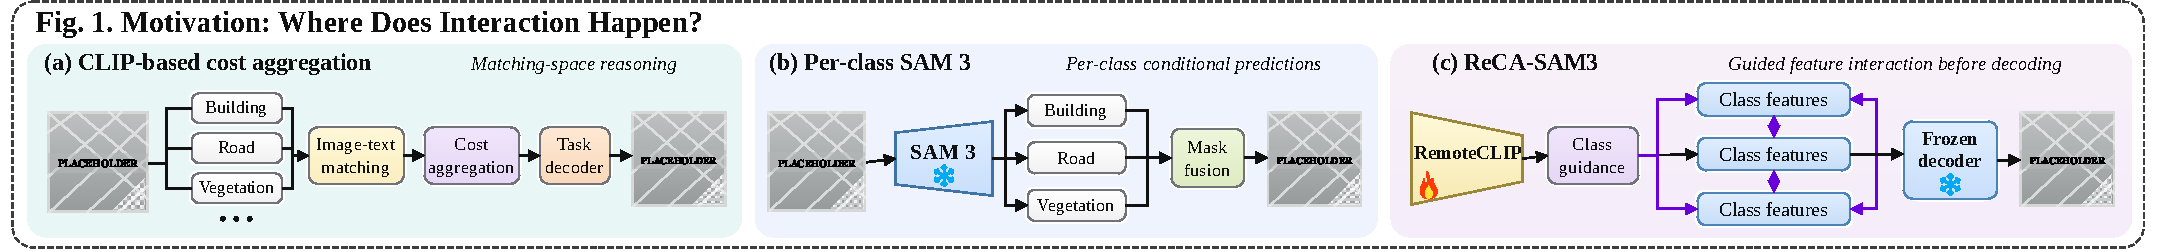
\includegraphics[width=\textwidth]{figures/motivation.pdf}
\caption{Motivation of ReCA-SAM3. Matching-space aggregation, per-class SAM 3 inference, and similarity-guided interaction of conditional features differ in where category context is incorporated. The gray image tiles are replaceable placeholders.}
\label{fig:motivation}
\end{figure*}


为此，本文提出 ReCA-SAM3。与对代价表征进行聚合并解码的管线相比，本文将每个类别提示的多模板图文相似度与稠密 RemoteCLIP 图像特征编码为指导特征，用于初始化独立的语义状态流。该状态与 SAM 3 类别条件特征共同构造注意力的查询和键，引导跨类别特征交换及提示内部的空间聚合；完整模型也通过注意力更新语义状态，使指导信息能够随特征上下文变化。随后，语义—细节融合模块连接更新后的 SAM 3 特征、原始条件特征与多尺度图像特征，复用冻结的解码路径。分割监督和原始软掩码蒸馏共同约束适配过程。

本文的方法贡献包括：
\begin{itemize}
\item 提出 RemoteCLIP 引导的双流特征聚合机制，将图文相似度转化为类别相关指导特征，并与 SAM 3 条件特征联合进行跨提示与提示内空间交互，在解码前建立领域语义引导的多类别上下文建模。
\item 设计面向冻结 SAM 3 解码路径的语义—细节融合模块，通过独立语义与细节分支及对齐后的方向响应融合连接聚合表征和原始空间特征，并结合参考软掩码约束构成特征适配方案。
\end{itemize}

\section{相关工作}

\subsection{遥感图文表征与开放词汇分割}
CLIP 通过图文对比学习建立视觉与语言的对应关系，为文本指定类别提供表征基础~\cite{radfordLearningTransferableVisual2021}。RemoteCLIP 将遥感检测框和分割掩码转换为图文样本，扩展遥感领域的图文预训练资源~\cite{liuRemoteCLIPVisionLanguage2024}。其领域表征能够提供语义先验，而将这类先验转化为像素级预测仍需要匹配、空间建模与解码设计。

GSNet 通过类别查询引导通用 CLIP 与遥感专用视觉特征融合，并以残差信息保留解码器恢复细节；其原始分割适配使用 LandDiscover50K~\cite{yeOpenVocabularyRemoteSensing2025}。RSKT-Seg 聚合多方向图文匹配，并通过 RemoteCLIP 等预训练编码器的中间特征进行领域知识迁移~\cite{liExploringEfficientOpenVocabulary2026}。Pi-Seg 在文本原型和稠密视觉特征中引入可学习扰动，以分割监督约束图文对齐~\cite{liPerturbationRegularizedOpenVocabularyRemote2026}。SegEarth-OV 则利用无标注遥感图像训练特征上采样器，并在推理时削弱局部特征中的全局偏置~\cite{liSegEarthOVTrainingFreeOpenVocabulary2025}。这些方法分别从表征、对齐或空间恢复入手。本文将遥感相似度编码为类别相关指导特征，使其参与 SAM 3 条件特征的注意力更新。

\subsection{SAM 3 与遥感提示适配}
SAM 3 支持以短名词短语或视觉示例指定待分割概念，并提供实例掩码及概念相关的语义响应~\cite{carionSAM3Segment2026}。SegEarth-OV3 逐类别查询 SAM 3，融合实例与语义响应，并使用概念存在分数抑制缺席类别~\cite{liSegEarthOV3ExploringSAM2026}。ProC-SAM3 构建离线类别提示池、缓存文本嵌入，并通过存在性和置信度校准融合响应~\cite{songPromptCalibratedSAM32026}。ROSE-SAM3 利用无标签图像上的冻结响应离线选择提示，并在预测时进行语义与实例协作~\cite{songROSESAM3ResponseOrientedPrompt2026}。RSGPNet 将初始预测掩码转换为几何框提示，再通过一致性验证细化结果~\cite{wangRSGPNetGeometricPrompting2026}。这些方法在保持模型参数冻结的同时调整提示或推理流程。ActiveSAM 则根据图像中的类别存在性裁剪活动词汇以减少解码开销~\cite{tienActiveSAMFastAccurate2026}。

本文使用 DLRSD 分割监督学习类别条件特征聚合，并在固定权重下进行目标域推理。

上述路径主要调整提示或预测输出。本文在解码前引入可学习的跨提示特征交互，采用源域监督训练聚合和融合模块，并部分适配 RemoteCLIP。SAM 3 参数保持冻结，原始语义路径仅在训练时提供软掩码约束；推理使用学生语义路径。参考掩码为特征适配提供原始空间响应的一致性约束。

\subsection{空间、类别与结构引导聚合}
CAT-Seg 将图文余弦相似度组织为代价体，交替进行空间和类别聚合，并通过上采样解码生成预测~\cite{choCATSegCostAggregation2024}。PCA-Seg 将两类聚合并行处理后融合~\cite{yinPCASegRevisitingCost2026}。RSKT-Seg 进一步设计空间及类别维度的高效代价融合~\cite{liExploringEfficientOpenVocabulary2026}。GeoSeg-OV 利用冻结视觉基础模型的结构特征，引导代价传播和多尺度解码，体现了语义匹配与空间结构协同建模的另一种方式~\cite{liuGeoSegOV2026}。

这些工作已经研究了空间与类别上下文，本文承接这一思想并改变交互对象与解码接口：模板级相似度经卷积和最终稠密 RemoteCLIP 特征融合后，形成每个提示的语义引导；它与当前 SAM 3 类别条件特征共同构造注意力的查询和键，而值始终来自条件特征。每个聚合块依次进行类间交互与共享权重的多尺度窗口聚合，仅残差更新条件特征。语义引导在各块间保持不变，并通过查询和键参与训练。最终送入冻结分割解码器的是聚合后的 SAM 3 特征经 SDF 融合得到的表征，相似度由此引导条件分割特征的适配。

\section{方法}
\subsection{框架概述}
ReCA-SAM3 由 SAM 3 特征提取、RemoteCLIP 语义引导、语义引导特征聚合和语义—细节融合四部分组成，如图~\ref{fig:overview} 所示。SAM 3 为各类别提示提取条件特征；RemoteCLIP 的模板级图文相似度与稠密图像特征经卷积融合，形成各提示的指导特征并初始化语义状态。该语义状态与 SAM 3 特征共同构造注意力，聚合模块在低分辨率网格上在每个块内依次建模提示间关系与提示内空间联系，再通过语义—细节融合（Semantic--Detail Fusion，SDF）将更新特征接入冻结的解码器。

\begin{figure*}[!tbp]
\centering
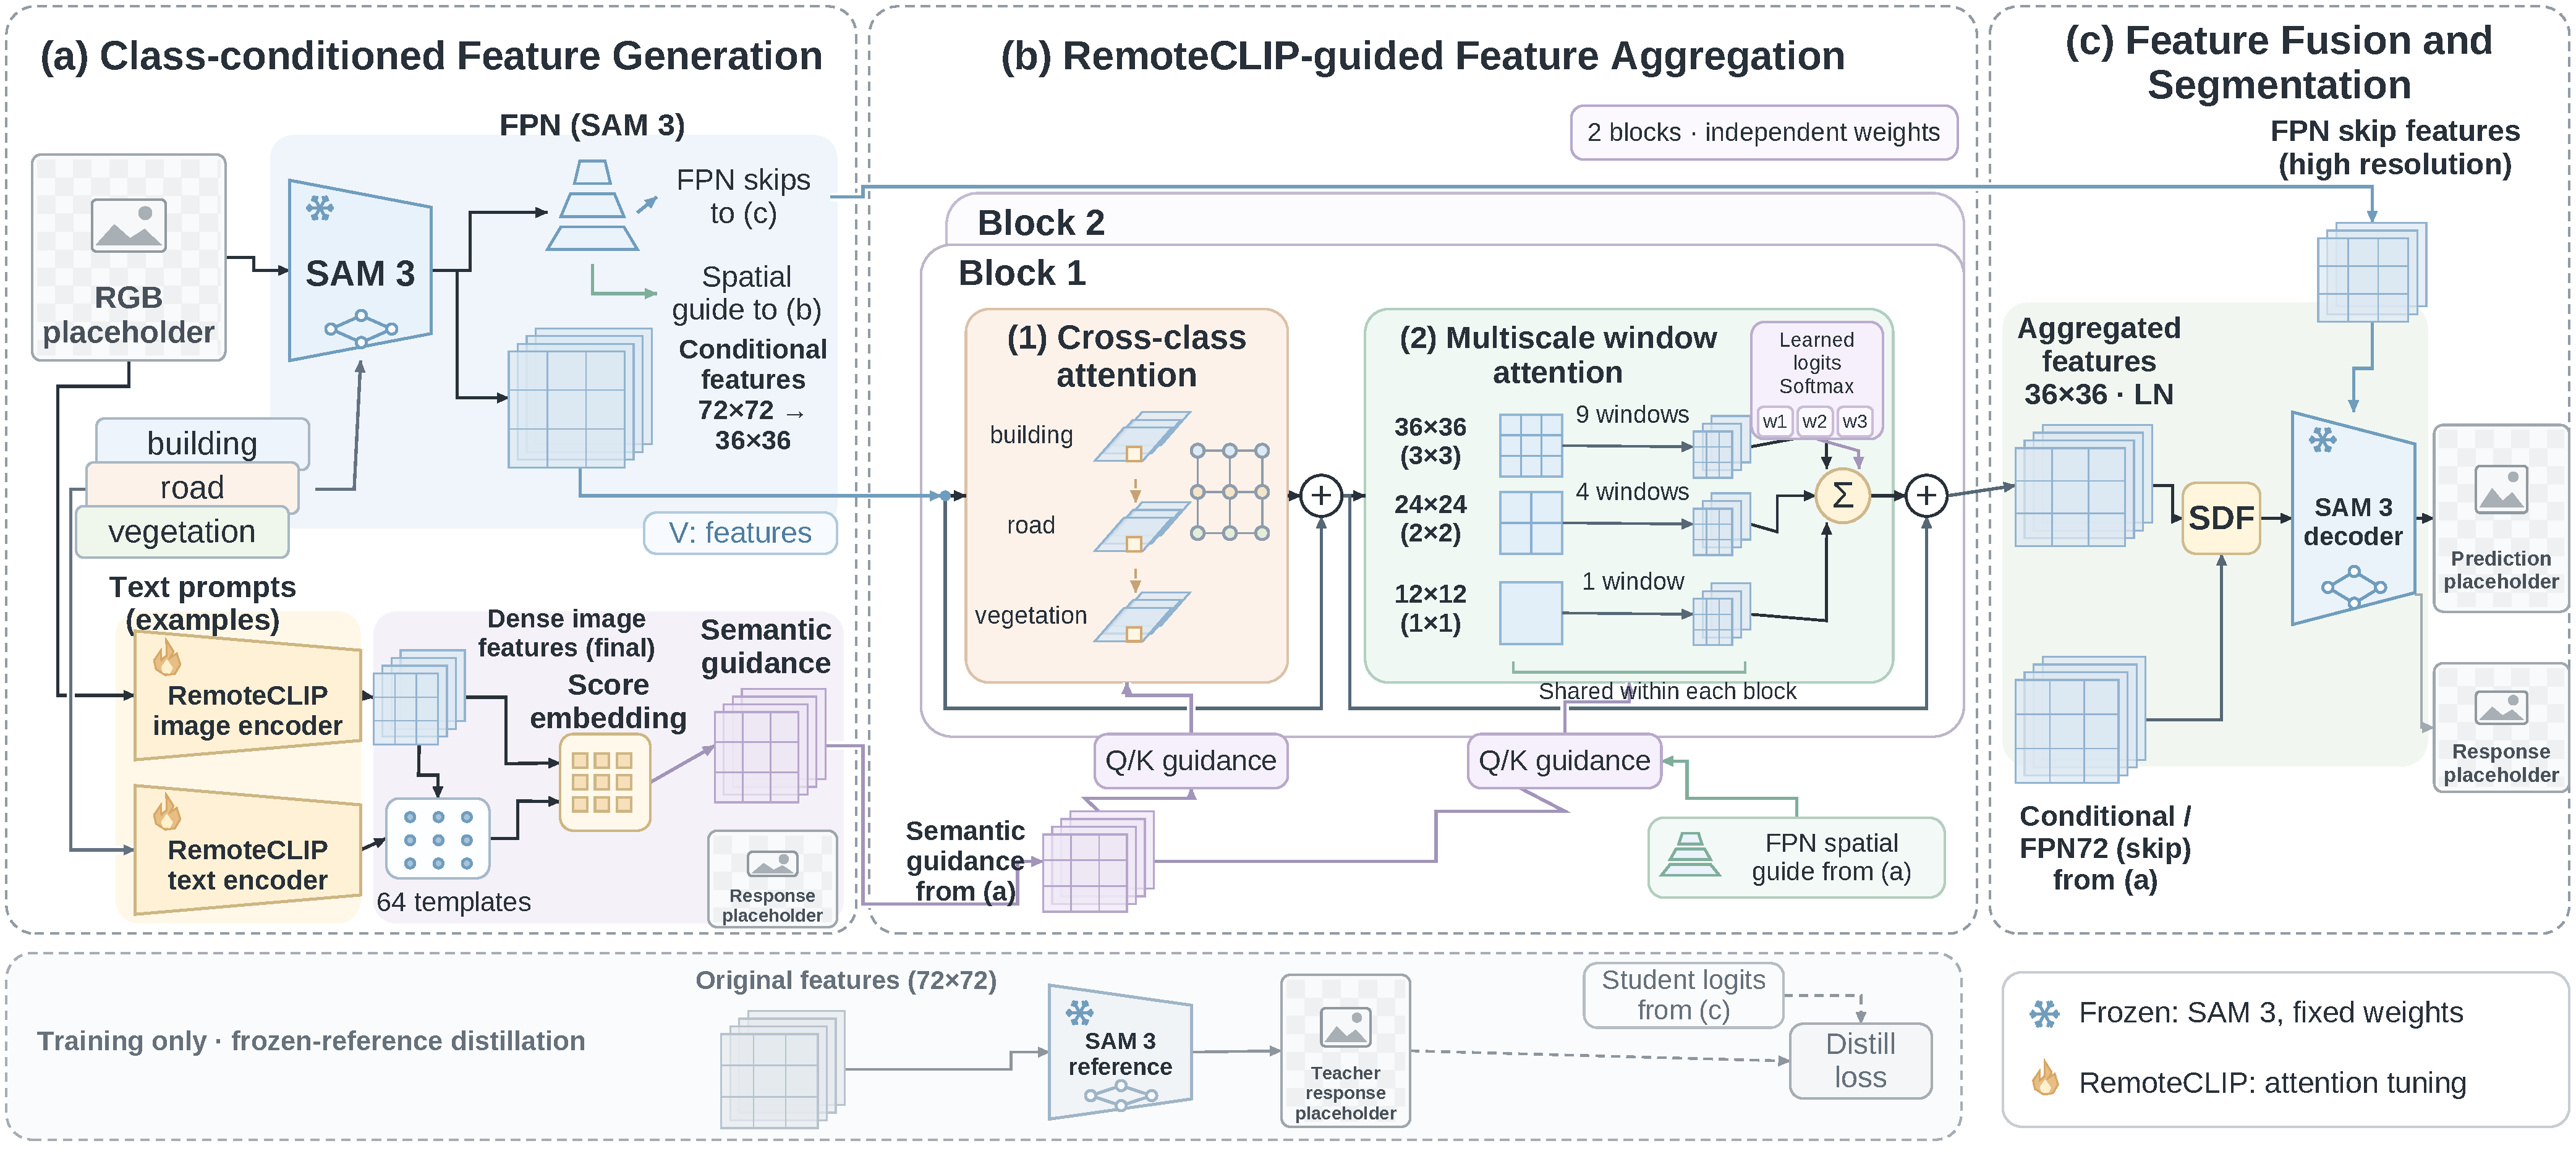
\includegraphics[width=\textwidth]{figures/overview.pdf}
\caption{Overview of ReCA-SAM3. (a) Class-conditioned feature extraction and RemoteCLIP guidance generation. (b) Two aggregation blocks with cross-class and shared multiscale window attention. (c) Semantic--Detail Fusion (SDF) and frozen decoding. The gray branch is used only for training-time distillation. Snowflakes and flames denote frozen modules and attention tuning, respectively. $\Sigma$ denotes weighted scale fusion, and $+$ denotes residual addition. Image and response tiles are placeholders.}
\label{fig:overview}
\end{figure*}


\subsection{任务定义与提示映射}
For an image $I$, let $\mathcal C=\{c_m\}_{m=0}^{M-1}$ denote the $M$ semantic classes represented in the model forward pass. Expanding aliases yields $P$ prompts $\{q_p\}_{p=1}^{P}$, with $\mu(p)\in\{0,\ldots,M-1\}$ mapping prompt $p$ to its forward class. Aliases share binary supervision but interact as separate prompt tokens. Background may participate in the forward pass or be restored afterward, so forward classes and evaluation labels are distinguished.

The frozen SAM 3 path supplies $E_p\in\mathbb R^{D\times72\times72}$ for each prompt, where $D=256$. This feature is obtained after the six-layer fusion encoder and the semantic head's prompt cross-attention. Image-level feature pyramid network (FPN) features are denoted by $J^s\in\mathbb R^{D\times s\times s}$ for $s\in\{72,144,288\}$, where $s$ specifies spatial resolution. The image backbone is evaluated once and reused across prompts.

Aggregation equations describe one image unless a batch index is shown. Flattening the $36\times36$ aggregation grid gives $N=36^2$ positions; each state has shape $P\times N\times D$. Cross-class attention acts along the expanded prompt axis, including aliases of the same class. Intra-class attention acts spatially within one prompt. Neither operation mixes images. Parameters are shared across prompt identities, allowing the candidate vocabulary size $P$ to vary.

\subsection{RemoteCLIP 语义引导}
RemoteCLIP provides local image--text alignment~\cite{liuRemoteCLIPVisionLanguage2024}. SAM 3 uses $1008\times1008$ inputs and RemoteCLIP uses $504\times504$ inputs, each with its own normalization. Let $U\in\mathbb R^{d_c\times36\times36}$ be the projected RemoteCLIP image features, with $d_c=768$, and $u_n$ its vector at position $n$. The vector $t_{pk}\in\mathbb R^{d_c}$ encodes prompt $p$ under template $k$, where $k=1,\ldots,K$ and $K=64$. Define $\mathcal N(v)=v/\max(\|v\|_2,\epsilon)$, where $v$ is a feature vector, $\|\cdot\|_2$ is its Euclidean norm, and $\epsilon=10^{-6}$. The template scores are
\begin{equation}
 C_{pkn}=\gamma\,\mathcal N(u_n)^\top\mathcal N(t_{pk}),
 \qquad \gamma=20.
 \label{eq:template_scores}
\end{equation}
Here $C_{pkn}$ is scaled cosine similarity, $\gamma$ is fixed, and $\top$ denotes transpose for the inner product. The scores of one prompt form $C_p\in\mathbb R^{K\times36\times36}$. Templates remain separate channels rather than being averaged into one text embedding.

The score embedding also incorporates dense image features:
\begin{equation}
\begin{aligned}
 A_p &= \phi_1(C_p),\\
 B_p &= \phi_2([\mathcal N(A_p);\mathcal N(U)]),\\
 S_p^0 &= \phi_3([\mathcal N(A_p);\mathcal N(B_p)]).
\end{aligned}
\label{eq:semantic_embedding}
\end{equation}
Brackets denote channel concatenation, and $\mathcal N$ acts independently at each position. The intermediate maps $A_p$ and $B_p$ have $D$ channels. Both $\phi_1$ and $\phi_2$ are a $1\times1$ convolution followed by eight-group GroupNorm and GELU; their input widths are $K$ and $D+d_c$, respectively. The function $\phi_3$ uses two $3\times3$ convolutions, each followed by GroupNorm and GELU, mapping $2D$ input channels to $D$ output channels. Parameters are shared across prompts. Stacking and flattening $S_p^0$ gives the initial semantic state $S^0\in\mathbb R^{P\times N\times D}$.

The similarity tensor in Eq.~\eqref{eq:template_scores} is converted into a class-specific guidance representation through Eq.~\eqref{eq:semantic_embedding}. Dense image features are shared across prompts, whereas the template-score input makes $S_p^0$ prompt dependent. For a class with several aliases, each expanded prompt retains its own guidance map. This similarity-derived semantic state remains unchanged during aggregation and supplies guidance to every attention step.

The feature state starts from the original conditional features:
\begin{equation}
 F_p^0=\mathcal D(E_p),
 \label{eq:feature_initialization}
\end{equation}
where $\mathcal D$ is bilinear resizing from $72\times72$ to $36\times36$. Stacking and flattening yields $F^0\in\mathbb R^{P\times N\times D}$. Superscript $0$ denotes initialization before aggregation: $S^0$ represents RemoteCLIP alignment information, whereas $F^0$ retains the SAM 3 conditional representation.

\subsection{语义引导特征聚合}
The encoder feature state passes through four complete aggregation blocks. Every block applies cross-class attention, regular-window attention, and shifted-window attention in that order. Each step adds a residual increment to the current encoder feature; the next step consumes the updated feature. The RemoteCLIP semantic state remains equal to its initialization throughout the stack. It is not detached, so gradients through queries and keys train its embedding module and the selected RemoteCLIP parameters. After all four blocks, a channel-wise LayerNorm produces the aggregated feature, denoted by $F^{\mathrm{agg}}$.

Cost-aggregation approaches contextualize image--text matching embeddings and decode the aggregated cost representation~\cite{choCATSegCostAggregation2024,liExploringEfficientOpenVocabulary2026}. Here similarity-derived semantics guide the aggregation of SAM 3 conditional segmentation features, which are then reconnected to the pretrained segmentation decoder through SDF. Blocks and attention steps have independent parameters and no additional feed-forward network.

\paragraph{Attention formulation.}
Each sub-update normalizes its current states along channels as $\bar S=\operatorname{LN}_S(S)$ and $\bar F=\operatorname{LN}_F(F)$. An optional spatial guide $G$ is independently normalized as $\bar G=\operatorname{LN}_G(G)$. Queries and keys use
\begin{equation}
 X_{\mathrm{qk}}=
 \begin{cases}
 [\bar S;\bar F], & \text{cross-class attention},\\
 [\bar S;\bar F;\bar G], & \text{window attention}.
 \end{cases}
 \label{eq:attention_input}
\end{equation}
At a fixed spatial position, cross-class attention takes $P$ tokens and an input width $2D$. Within a fixed prompt and window, window attention takes $w^2$ tokens and width $3D$, with window side length $w=12$. Image-level guides are broadcast across prompts before window partitioning.

Only encoder features supply values: $\bar R=\bar F$, where $\bar R$ denotes the normalized value input. Head $h=1,\ldots,n_h$ computes
\begin{equation}
\begin{aligned}
 Q_h &= X_{\mathrm{qk}}W_h^Q+b_h^Q,\\
 K_h &= X_{\mathrm{qk}}W_h^K+b_h^K,\\
 V_h &= \bar R W_h^V+b_h^V,\\
 A_h &= \operatorname{Drop}_a\!\left[
 \operatorname{softmax}_{\mathrm{key}}\!\left(
 \frac{Q_hK_h^\top}{\sqrt{d_h}}+B_h+M_{\mathrm{sh}}
 \right)\right].
\end{aligned}
\label{eq:attention_heads}
\end{equation}
Here $n_h=8$ is the head count and $d_h=D/n_h=32$ is the head width. The matrices $Q_h,K_h,V_h$ are queries, keys, and values. The learned matrices $W_h^Q,W_h^K,W_h^V$ and biases $b_h^Q,b_h^K,b_h^V$ define affine projections, broadcasting biases across tokens. For cross-class/window attention, $W_h^Q$ and $W_h^K$ have size $2D\times d_h$/$3D\times d_h$; $W_h^V$ has size $D\times d_h$, and each head bias has $d_h$ entries. Softmax normalizes key tokens separately for each query. The matrix $B_h$ is a learned window-relative position bias and is zero for cross-class attention. The mask $M_{\mathrm{sh}}$ has large negative entries for disallowed cyclic-boundary interactions in shifted windows; it is zero for regular windows and cross-class attention. The function $\operatorname{Drop}_a$ applies dropout to attention weights, giving $A_h$.

The residual increment is
\begin{equation}
 \Delta R=\operatorname{Drop}_o\!\left(
 [A_1V_1;\ldots;A_{n_h}V_{n_h}]W^O+b^O
 \right),
 \label{eq:attention_output}
\end{equation}
where head outputs are concatenated along channels, $W^O\in\mathbb R^{D\times D}$ and $b^O\in\mathbb R^D$ form the output projection, and $\operatorname{Drop}_o$ is output dropout. Both dropout operations use probability 0.1 during training and are disabled for inference. The raw target state is denoted by $R$, and its increment $\Delta R$ has the same shape. A guide affects Q/K but contributes neither values nor a direct residual. Cross-class, regular-window, shifted-window steps and different blocks each have separate normalization and projection parameters.

\paragraph{Cross-class and window updates.}
Cross-class attention forms a prompt-by-prompt matrix at every spatial position and adds its output to the encoder feature state. Window attention then applies two successive feature updates, first without a shift and then with a six-pixel cyclic shift. The image-level guide is the bilinearly downsampled SAM 3 FPN72 feature. This guide is computed once, broadcast across prompts, and concatenated into window queries and keys only. Regular and shifted windows retain learned relative position bias; the shifted step also masks cyclic-boundary interactions and restores output coordinates before residual addition. RemoteCLIP intermediate features are still extracted and cached by the implementation but are not inputs to these attention updates.

\subsection{语义—细节融合与解码}
SDF reconnects aggregated features to the original decoder at $72\times72$, as illustrated in Fig.~\ref{fig:sdf}. With $\mathcal U$ denoting bilinear upsampling from $36\times36$ to $72\times72$, prompt $p$ has branch inputs
\begin{equation}
\begin{aligned}
 A_p^{72} &= \mathcal U(F_p^{\mathrm{agg}}),\\
 X_{s,p} &= \Pi_s(A_p^{72})+\Pi_E(E_p),\\
 X_{d,p} &= \Pi_d(A_p^{72})+\Pi_J(J^{72}).
\end{aligned}
\label{eq:sdf_inputs}
\end{equation}
Here $F_p^{\mathrm{agg}}$ is the reshaped feature slice, $A_p^{72}$ its upsampled map, and $X_{s,p},X_{d,p}$ the semantic/detail branch inputs. Each of $\Pi_s,\Pi_E,\Pi_d,\Pi_J$ is an independent $1\times1$ convolution plus eight-group GroupNorm. All maps have $D$ channels; the projected image-level $J^{72}$ is broadcast over prompts. The two branches retain separate access to original conditional features and image-level spatial features.

\begin{figure*}[!tbp]
\centering
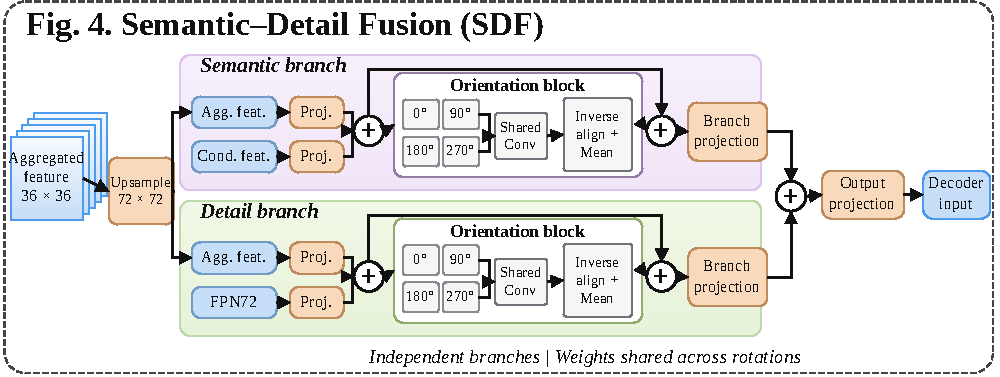
\includegraphics[width=\textwidth]{figures/sdf.pdf}
\caption{Semantic--Detail Fusion. A common upsampled aggregation feature feeds two independently parameterized branches. Each branch combines independently projected inputs, averages inverse-aligned convolutional responses over four orientations, and adds a residual. Branch projections are added and followed by a final output projection.}
\label{fig:sdf}
\end{figure*}


Let $\mathcal R_b(X)=X+g_b(X)$ denote the single-direction residual branch operation. Here $b$ indexes the semantic or detail branch, $X$ is its input feature map, and $g_b$ is its independently parameterized convolution block.

Each branch applies its independent convolution block once in the original orientation and adds the result to its input. The block comprises a $3\times3$ convolution, GroupNorm, GELU, a $1\times1$ convolution, and GroupNorm. There is no feature rotation or averaging across orientations.

The fused decoder feature and student logits are
\begin{equation}
\begin{aligned}
 D_p={}&\Psi_o\bigl(\Psi_s(\mathcal R_s(X_{s,p}))\\
       &\hspace{3.4em}+\Psi_d(\mathcal R_d(X_{d,p}))\bigr),\\
 z_p={}&\mathcal H(D_p;J^{144},J^{288}).
\end{aligned}
\label{eq:sdf_decode}
\end{equation}
Here $D_p\in\mathbb R^{D\times72\times72}$ is the decoder feature and $z_p\in\mathbb R^{288\times288}$ is the prompt logit map. The independent $1\times1$ convolutions $\Psi_s,\Psi_d,\Psi_o$ have no additional output activation or normalization. The operator $\mathcal H$ is the shared frozen SAM 3 Pixel Decoder and semantic head: its last FPN input is replaced by $D_p$, while $J^{144}$ and $J^{288}$ are retained. Its parameters remain fixed, but the student computation is differentiable with respect to $D_p$, allowing gradients to reach SDF and aggregation.

\subsection{训练目标}
A training batch contains $B$ images indexed by $b=1,\ldots,B$. The forward-space label map $y_b(x)$ is resized by nearest-neighbor interpolation to the $288\times288$ logit grid; $x$ denotes a position on that grid. Let $\Omega_b=\{x:y_b(x)\ne255\}$ be the valid-pixel set. Prompt targets and groups are
\begin{equation}
\begin{aligned}
 Y_{bp}(x)&=\mathbf 1[y_b(x)=\mu(p)],\\
 \mathcal P_b^+&=\{p:\exists x\in\Omega_b,\ Y_{bp}(x)=1\},\\
 \mathcal P_b^-&=\{1,\ldots,P\}\setminus\mathcal P_b^+.
\end{aligned}
\label{eq:supervision_sets}
\end{equation}
The indicator $\mathbf 1[\cdot]$ equals one for a true condition and zero otherwise. The sets $\mathcal P_b^+,\mathcal P_b^-$ contain present/absent expanded prompts; $\setminus$ is set difference. Presence comes from valid ground truth, not a predicted presence score. Aliases share targets through $\mu$ but remain separate terms in prompt-group means.

For logit $z$ and binary or soft target $y\in[0,1]$, define binary cross-entropy (BCE) by
\begin{equation}
 \ell_{\mathrm{BCE}}(z,y)=\log(1+\exp(z))-yz.
 \label{eq:bce_definition}
\end{equation}
Here $\log$ is the natural logarithm. The implementation uses numerically stable BCE with logits. Let $z_{bp}(x)$ be the student logit for image $b$, prompt $p$, and position $x$. Per-prompt and per-image group means are
\begin{equation}
\begin{aligned}
 L_{bp}&=\frac{\sum_{x\in\Omega_b}\ell_{\mathrm{BCE}}(z_{bp}(x),Y_{bp}(x))}
                  {\max(1,|\Omega_b|)},\\
 L_b^+&=\frac{\sum_{p\in\mathcal P_b^+}L_{bp}}{\max(1,|\mathcal P_b^+|)},\\
 L_b^-&=\frac{\sum_{p\in\mathcal P_b^-}L_{bp}}{\max(1,|\mathcal P_b^-|)}.
\end{aligned}
\label{eq:group_means}
\end{equation}
Vertical bars denote cardinalities. Empty sums are zero, including images with no valid pixels. The group denominators use all prompts before decoding chunks are formed. Positive and negative pixels inside one prompt receive equal pixel weights; the balancing acts between present and absent prompt groups.

A sole nonempty group receives full weight through
\begin{equation}
 \alpha_b=
 \begin{cases}
 \alpha, & |\mathcal P_b^+|>0\ \text{and}\ |\mathcal P_b^-|>0,\\
 1, & |\mathcal P_b^+|>0\ \text{and}\ |\mathcal P_b^-|=0,\\
 0, & \text{otherwise},
 \end{cases}
 \label{eq:group_weight}
\end{equation}
where $\alpha\in[0,1]$ is the configured present-group weight and $\alpha_b$ its effective per-image value. The segmentation loss is
\begin{equation}
 \mathcal L_{\mathrm{seg}}=\frac{1}{B}\sum_{b=1}^{B}
 [\alpha_b L_b^+ +(1-\alpha_b)L_b^-],
 \label{eq:segmentation_loss}
\end{equation}
with $\alpha=0.8$ in the current configuration. All $B$ images enter the batch mean; all-ignore images contribute zero. Normalization is over expanded prompts, so classes with more aliases are not reduced to one equally weighted class term.

\paragraph{Frozen-reference distillation.}
The reference branch applies the same frozen decoder to the original conditional feature:
\begin{equation}
\begin{aligned}
 z^{\mathrm t}_{bp}&=\mathcal H(E_{bp};J_b^{144},J_b^{288}),\\
 r^{\mathrm t}_{bp}(x)&=\operatorname{sg}(\sigma(z^{\mathrm t}_{bp}(x))).
\end{aligned}
\label{eq:teacher_target}
\end{equation}
The batch index is restored on $E$ and $J$. The map $z^{\mathrm t}_{bp}$ is the reference logit map, $r^{\mathrm t}_{bp}$ its soft target, $\sigma(z)=1/(1+\exp(-z))$ the sigmoid, and $\operatorname{sg}$ stop-gradient. This branch is evaluated without an autograd graph. Its loss is
\begin{equation}
\begin{aligned}
 N_{\mathrm{KD}}&=\sum_{b=1}^{B}|\mathcal P_b^+|\,|\Omega_b|,\\
 \mathcal L_{\mathrm{KD}}&=\frac{1}{\max(1,N_{\mathrm{KD}})}\sum_{b=1}^{B}
 \sum_{p\in\mathcal P_b^+}\sum_{x\in\Omega_b}
 \ell_{\mathrm{BCE}}(z_{bp}(x),r^{\mathrm t}_{bp}(x)).
\end{aligned}
\label{eq:distillation_loss}
\end{equation}
The denominator $N_{\mathrm{KD}}$ counts valid pixels over all present image--prompt pairs in the batch. Distillation is therefore a global pixel mean, unlike the per-image group balancing of Eq.~\eqref{eq:segmentation_loss}. It is zero when $N_{\mathrm{KD}}=0$. Absent prompts and ignored pixels are excluded, and no boundary ring is constructed.

The total objective is
\begin{equation}
 \mathcal L=\lambda_{\mathrm{seg}}\mathcal L_{\mathrm{seg}}
            +\lambda_{\mathrm{KD}}\mathcal L_{\mathrm{KD}},
 \label{eq:total_loss}
\end{equation}
where $\mathcal L$ denotes the training loss and $\lambda_{\mathrm{seg}},\lambda_{\mathrm{KD}}$ are fixed nonnegative coefficients, currently 1 and 0.5. The optional Dice term is disabled. Aggregation and SDF are trained; SAM 3 remains frozen. RemoteCLIP image/text branches update attention Q/V projections and positional parameters while keeping stochastic layers in evaluation mode. Prompt chunks share the full-batch denominators in Eqs.~\eqref{eq:group_means} and~\eqref{eq:distillation_loss}; summing their contributions implements the same objective as decoding all prompts together.

\subsection{推理与标签恢复}
Inference evaluates only the student path, without reference decoding or instance/presence fusion. Aliases are merged after sigmoid on the decoded grid:
\begin{equation}
 r_m(x)=\max_{p:\mu(p)=m}\sigma(z_p(x)),
 \qquad m=0,\ldots,M-1.
 \label{eq:alias_merge}
\end{equation}
The response $r_m(x)$ belongs to forward class $m$ at position $x$; the maximum ranges over its aliases. Aliases are merged at prediction, whereas the $K$ template channels remain separate during prior construction. For datasets enabling background handling, the student threshold gives
\begin{equation}
 \widetilde r_m(x)=
 \begin{cases}
 r_m(x)\,\mathbf 1[r_m(x)\ge\tau_s], & e_{\mathrm{bg}}=1,\\
 r_m(x), & e_{\mathrm{bg}}=0.
 \end{cases}
 \label{eq:student_filter}
\end{equation}
Here $\widetilde r_m$ is the filtered response, $e_{\mathrm{bg}}\in\{0,1\}$ indicates enabled background handling, and $\tau_s\in[0,1]$ is the student probability threshold. Disabling the threshold gives the identity. Without background, all class scores are retained for argmax.

Define the winning forward class $m^*(x)=\arg\max_m\widetilde r_m(x)$ and score $r^*(x)=\max_m\widetilde r_m(x)$. Let $\rho$ map forward indices to evaluation labels and $c_{\mathrm{bg}}$ denote the background label. The prediction is
\begin{equation}
 \widehat y(x)=
 \begin{cases}
 c_{\mathrm{bg}}, & e_{\mathrm{bg}}=1\ \text{and}\ r^*(x)\le\tau_b,\\
 \rho(m^*(x)), & \text{otherwise}.
 \end{cases}
 \label{eq:label_restore}
\end{equation}
The map $\widehat y$ is in evaluation label space, and $\tau_b\in[0,1]$ is the background fallback threshold; its first case is omitted when fallback is disabled. If background was excluded from the forward pass, $\rho$ restores its reserved index; otherwise indices are unchanged. Argmax ties select the first forward class index. The current thresholds are $\tau_s=0.5$ and $\tau_b=0$, and test-time augmentation is disabled.

\FloatBarrier
\section{实验}
\subsection{数据集与评价指标}
本文采用 RSKT-Seg 的八数据集评测集合：DLRSD、iSAID、LoveDA、Potsdam、Vaihingen、UAVid、UDD5 和 VDD~\cite{liExploringEfficientOpenVocabulary2026}。DLRSD 保留 OVRSISBench 发布包中的 5601 张训练图像与 1401 张验证图像，分别用于单源监督适配与源域评测。LoveDA 验证集用于模型选择，作为开发域；其余六个数据集用于目标域评测。数据角色、类别数、展开提示数及预测过滤阈值见表~\ref{tab:dataset_protocol}。
% Generated from paper/data; do not hand-edit numeric cells.
\begin{table*}[!tbp]
\centering
\caption{Dataset roles, class prompts, and prediction filtering.}
\label{tab:dataset_protocol}
\footnotesize
\setlength{\tabcolsep}{2pt}
\begin{tabularx}{\linewidth}{@{}L{0.14\linewidth}L{0.10\linewidth}*{2}{C}L{0.20\linewidth}C@{}}
\toprule
Dataset & Role & Classes & Prompts & Background & \shortstack{Prediction\\threshold}\\
\midrule
DLRSD & Source & 17 & 17 & None & Off\\
iSAID & Target & 15 & 15 & Ignored & Off\\
LoveDA & Dev. & 7 & 7 & background & 0.5\\
Potsdam & Target & 6 & 7 & clutter & 0.0\\
Vaihingen & Target & 6 & 7 & clutter & 0.0\\
UAVid & Target & 7 & 7 & background & 0.3\\
UDD5 & Target & 5 & 5 & background & 0.4\\
VDD & Target & 7 & 9 & background & 0.5\\
\bottomrule
\end{tabularx}
\par\vspace{3pt}
\begin{minipage}{\linewidth}
\footnotesize Source: DLRSD adaptation and source-domain evaluation. Dev.: LoveDA checkpoint selection. Target: independent target-domain evaluation. Every configured class participates in forward inference. Aliases expand the prompt count without changing the semantic class count. Off means filtering is inactive. The same prompts and dataset-specific threshold are used for all local methods and variants. Background fallback uses a separate threshold of 0.0.
\end{minipage}
\end{table*}


所有数据集均对配置中的全部类别执行前向，背景或 clutter 作为已配置类别时也参与预测。同义词展开为独立文本提示，并在输出端按原语义类别逐像素取最大值合并；因此提示数可以多于类别数。Potsdam 与 Vaihingen 的道路类别使用 road 和 pavement，VDD 的屋顶类别使用 roof、rooftop 和 building top。UAVid 合并 moving car 与 static car 为 car，采用含背景的七类评测；LoveDA 同样采用含背景七类，iSAID 背景像素忽略，DLRSD 不另设背景。忽略值统一为 255。LoveDA 原始标签 1--7 仅转换一次为 0--6，原始 0 转为忽略值，前向与评测不再额外删除背景或平移编号。

主要指标为平均交并比（mIoU），辅助保存平均类别准确率（mAcc）与逐类交并比（IoU）。并集为零的类别按评测器规则排除，同时记录有效类别数。跨数据集评测用于考察迁移表现；对训练类别与目标类别的语义重叠另行核对，不将全部目标类别直接视为严格未见类别。

\subsection{实现细节与统一评测协议}
SAM 3 输入为 1008×1008，RemoteCLIP 输入为 504×504；每个文本提示使用 64 个固定模板。提示条件特征从 72×72 下采样至 36×36，经过两个聚合块。每块先在同一空间位置沿完整提示集合执行类间注意力，再并行计算 36×36、24×24 和 12×12 三个尺度的类内注意力。各分支均使用 12×12 普通窗口，窗口数依次为 9、4 和 1，最小尺度覆盖全图。同一块的三尺度分支共享注意力参数，不同块分别学习参数；三路更新对齐至 36×36 后，以每块独立学习的三个 Softmax 权重融合并残差更新特征。融合参数从零初始化，对应初始等权。类内注意力保留 SAM 3 FPN 引导，RemoteCLIP 仅通过 score embedding 提供图文语义引导，中间层图像特征不参与聚合。注意力使用八个头与 0.1 dropout，最终在 72×72 上执行一次 256 通道单方向语义--细节融合（SDF），提示解码分块大小为 4。

SAM 3 特征提取、提示编码、条件编码器、Pixel Decoder 与分割头冻结；聚合、score embedding 及 SDF 参数训练。主模型对 RemoteCLIP 图像和文本编码器执行 attention 微调。优化采用 AdamW，基础学习率为 \texttt{1e-4}，RemoteCLIP 参数组使用 0.01 倍率。批量为 4，总预算为 10000 步，其中前 500 步线性预热，后 9500 步按参数组比例余弦衰减，最低学习率为各组目标学习率的 0.01 倍，梯度裁剪阈值为 0.01。每 1000 步保存并完整验证。训练使用自动混合精度、随机裁剪或整图缩放、随机直角旋转、颜色增强与水平翻转，两个图像分支与标签共享空间变换。

主分割二元交叉熵（BCE）先对每图每提示的有效像素平均，再分别平均存在与不存在提示，默认组权重为 0.8 与 0.2。Dice 权重为零。蒸馏采用冻结 SAM 3 教师的软概率，仅监督存在提示的有效标注像素，固定权重为 0.5；教师解码仅在训练需要蒸馏时执行，评测只运行学生路径。

每个训练变体在同一预算内按 LoveDA 七类 mIoU 选择一份权重，并用于该次训练的全部数据集和全部表格，不按目标数据集分别选择最优 checkpoint。各变体使用相同随机种子集合；多种子结果报告均值与样本标准差，单种子结果只报告单次值。主模型在不同消融表中的结果共用同一次评测，不重复训练。验证直接缩放至 1008×1008，保持当前协议的非等比缩放，默认关闭测试时增强。同一数据集内固定类别提示、标签映射和过滤阈值，不逐变体调参。先合并同义提示，再将低于预测阈值的类别概率置零，阈值边界保留；无背景数据集跳过该过滤。背景回填阈值独立设为 0.0。

\subsection{与现有方法的比较}
% Generated from paper/data; do not hand-edit numeric cells.
\begin{table*}[!tbp]
\centering
\caption{Semantic segmentation results on eight remote sensing datasets (mIoU, \%).}
\label{tab:main_rskt8}
\footnotesize
\setlength{\tabcolsep}{2pt}
\begin{tabularx}{\linewidth}{@{}L{0.25\linewidth}L{0.08\linewidth}*{9}{C}@{}}
\toprule
Method & \shortstack{Adaptation\\data} & DLRSD & \shortstack{iSAID\\15 cls.\\IgnBG} & \shortstack{iSAID\\16 cls.\\BG} & LoveDA & Potsdam & Vaihingen & UAVid & UDD5 & VDD\\
\midrule
\multicolumn{11}{l}{\textbf{Training on remote sensing segmentation data}}\\
SCAN~\cite{liu2024openvocabularysegmentationsemanticassistedcalibration} & DLRSD & 52.42 & 44.28 & -- & 23.17 & 27.45 & 15.23 & 20.28 & 34.14 & 29.24\\
SAN~\cite{xu2023adapternetworkopenvocabularysemantic} & DLRSD & 86.45 & 49.56 & -- & 25.33 & 37.25 & 39.22 & 23.53 & 37.23 & 35.83\\
SED~\cite{xie2024sedsimpleencoderdecoderopenvocabulary} & DLRSD & 87.68 & 51.23 & -- & 24.55 & 29.35 & 39.02 & 21.33 & 35.73 & 32.53\\
CAT-Seg~\cite{choCATSegCostAggregation2024} & DLRSD & 88.68 & 53.34 & -- & 28.64 & 35.75 & 42.30 & 25.73 & 40.24 & 39.14\\
OVRS~\cite{caoOVRSHighResolution2025} & DLRSD & 88.85 & 52.65 & -- & 31.53 & 36.44 & 43.50 & 24.13 & 40.82 & 37.23\\
GSNet~\cite{yeOpenVocabularyRemoteSensing2025} & DLRSD & 86.02 & 53.73 & -- & 32.52 & 37.85 & 44.13 & 24.22 & 40.92 & 37.34\\
RSKT-Seg~\cite{liExploringEfficientOpenVocabulary2026} & DLRSD & 93.49 & 54.32 & -- & 33.23 & 38.44 & 42.69 & 25.72 & 42.10 & 39.69\\
Pi-Seg~\cite{liPerturbationRegularizedOpenVocabularyRemote2026} & DLRSD & -- & -- & -- & 39.00 & 35.33 & 44.18 & 33.58 & 59.08 & 47.73\\
UGDMoE~\cite{quUGDMoE2026} & DLRSD & 93.35 & -- & -- & 34.17 & 38.21 & 44.92 & 26.85 & 43.78 & 40.12\\
SkySense-O~\cite{zhuSkySenseOOpenWorldRemote2025a} & Sky-SA & -- & -- & -- & 38.30 & 54.10 & 51.64 & -- & -- & --\\
ReCA-SAM3 & DLRSD & -- & -- & -- & -- & -- & -- & -- & -- & --\\
\midrule
\multicolumn{11}{l}{\textbf{Training-free}}\\
SCLIP~\cite{wang2024scliprethinkingselfattentiondense} & None & -- & -- & 16.10 & 30.40 & 39.60 & 35.90 & 31.40 & 38.70 & 37.90\\
ClearCLIP~\cite{lan2024clearclipdecomposingcliprepresentations} & None & -- & -- & 18.20 & 32.40 & 42.00 & 36.20 & 36.20 & 41.80 & 39.30\\
ProxyCLIP~\cite{lan2024proxyclipproxyattentionimproves} & None & -- & -- & 21.80 & 34.30 & 49.00 & 47.50 & 35.80 & 40.80 & 47.80\\
CorrCLIP~\cite{zhang2025corrclipreconstructingpatchcorrelations} & None & -- & -- & 25.50 & 36.90 & 51.90 & 47.00 & 38.30 & 46.10 & 47.30\\
SegEarth-OV~\cite{liSegEarthOVTrainingFreeOpenVocabulary2025} & None & -- & -- & 21.7 & 36.9 & 47.1 & 29.1 & 42.5 & 50.6 & 45.3\\
ConInfer~\cite{chen2026coninfercontextawareinferencetrainingfree} & None & -- & -- & -- & 39.33 & 49.99 & 31.37 & 46.40 & 46.86 & 50.29\\
ActiveSAM~\cite{tienActiveSAMFastAccurate2026} & None & -- & -- & 28.30 & 41.10 & 40.60 & 45.10 & 53.30 & 72.10 & 62.20\\
SegEarth-OV3~\cite{liSegEarthOV3ExploringSAM2026} & None & -- & -- & 27.6 & 47.4 & 57.8 & 60.8 & 54.7 & 71.7 & 64.5\\
RSGPNet~\cite{wangRSGPNetGeometricPrompting2026} & None & -- & -- & -- & 47.80 & 59.70 & 61.10 & -- & 71.00 & --\\
GLoP-SAM3~\cite{liuGLoPSAM3DualPostprocessing2026} & None & -- & -- & -- & 46.20 & 57.90 & 62.20 & 55.40 & 72.60 & 64.70\\
ProC-SAM3~\cite{songPromptCalibratedSAM32026} & None & -- & -- & 29.5 & 46.1 & 58.8 & 64.5 & 60.0 & 73.4 & 67.5\\
ROSE-SAM3~\cite{songROSESAM3ResponseOrientedPrompt2026} & Unlabeled & -- & -- & 35.10 & 48.70 & 58.90 & 65.30 & 59.90 & 73.70 & 67.50\\
SAM 3 Semantic-only & None & -- & -- & -- & -- & -- & -- & -- & -- & --\\
SAM 3 Semantic $\times$ Presence & None & -- & -- & -- & -- & -- & -- & -- & -- & --\\
\bottomrule
\end{tabularx}
\par\vspace{3pt}
\begin{minipage}{\linewidth}
\footnotesize Literature results are taken from the cited papers. SCAN, SAN, SED, CAT-Seg, OVRS and GSNet use the results reported by RSKT-Seg~\cite{liExploringEfficientOpenVocabulary2026}; SCLIP, ClearCLIP, ProxyCLIP and CorrCLIP use SegEarth-OV3~\cite{liSegEarthOV3ExploringSAM2026}. ActiveSAM uses the reproduction in ProC-SAM3~\cite{songPromptCalibratedSAM32026}; GLoP-SAM3 is quoted from ROSE-SAM3~\cite{songROSESAM3ResponseOrientedPrompt2026}. IgnBG: background ignored; BG: background included. --: not reported.\par iSAID references (protocol unspecified; mIoU, \%): Pi-Seg: 53.50; UGDMoE: 54.38; SkySense-O: 43.92; ConInfer: 20.08; GLoP-SAM3: 28.00.
\end{minipage}
\end{table*}

表~\ref{tab:main_rskt8} 在本地统一协议区域设置两个原始 SAM 3 基线与完整 ReCA-SAM3。Semantic-only 直接输出原始 SAM 3 语义概率；Semantic $\times$ Presence 执行原始语义与实例查询流程，将每个提示的语义概率乘一次对应的 presence 概率，再按语义类别合并同义提示，不融合实例掩码。两个基线使用同一原始 SAM 3 预训练权重，无 DLRSD 分割适配；完整模型使用 DLRSD 适配。所有本地行采用相同输入、类别提示、标签、背景和后处理设置。

文献区域保留已登记来源的原报告值。CAT-Seg 与 GSNet 的 iSAID 单源设置来自 RSKT-Seg Table 1，而非本地运行其官方权重~\cite{liExploringEfficientOpenVocabulary2026}；GSNet 原论文与官方训练设置使用 LandDiscover50K~\cite{yeOpenVocabularyRemoteSensing2025}。RSKT-Seg、Pi-Seg、SegEarth-OV、SegEarth-OV3 和 ProC-SAM3 各自保留已核对版本及来源，不按列混入其他论文的复现值。训练资源、类别映射、裁块、图像几何与阈值未完全一致的文献结果不参与同条件排名，也不与本地结果混算跨域平均。

\subsection{LoveDA 逐类分析}
% Generated from paper/data; do not hand-edit numeric cells.
\begin{table*}[!tbp]
\centering
\caption{Per-class IoU and mIoU on LoveDA (\%).}
\label{tab:loveda_per_class}
\footnotesize
\setlength{\tabcolsep}{2pt}
\begin{tabularx}{\linewidth}{@{}L{0.25\linewidth}*{8}{C}@{}}
\toprule
Method & Background & Building & Road & Water & Barren & Forest & Agricultural & mIoU\\
\midrule
ReCA-SAM3 & -- & -- & -- & -- & -- & -- & -- & --\\
SAM 3 Semantic-only & -- & -- & -- & -- & -- & -- & -- & --\\
SAM 3 Semantic $\times$ Presence & -- & -- & -- & -- & -- & -- & -- & --\\
\bottomrule
\end{tabularx}
\par\vspace{3pt}
\begin{minipage}{\linewidth}
\footnotesize All seven classes, including background, contribute to mIoU. Each row reuses its LoveDA evaluation and checkpoint from the main comparison. LoveDA is the development domain. -- denotes unavailable results.
\end{minipage}
\end{table*}

表~\ref{tab:loveda_per_class} 为两个原始 SAM 3 基线与完整模型分别记录 background、building、road、water、barren、forest、agricultural 的 IoU 和七类 mIoU。该表复用主对比中的 LoveDA 评测记录，用于分析各语义类别的变化。LoveDA 已用于模型选择，逐类结果属于开发域分析；目标域泛化依据其他独立目标数据集评测。

\subsection{核心结构与监督消融}
% Generated from paper/data; do not hand-edit numeric cells.
\begin{table}[!htbp]
\centering
\caption{Ablation of feature aggregation, fusion, and supervision (mIoU, \%).}
\label{tab:ablation_core}
\small
\setlength{\tabcolsep}{2pt}
\begin{tabularx}{\linewidth}{@{}L{0.48\linewidth}*{3}{C}@{}}
\toprule
Variant & LoveDA & Potsdam & UAVid\\
\midrule
Full & -- & -- & --\\
SAM 3 adapter & -- & -- & --\\
Diagonal cross-prompt attention & -- & -- & --\\
Encoder feature updates only & -- & -- & --\\
w/o intra-class aggregation & -- & -- & --\\
w/o initial semantic prior & -- & -- & --\\
Simple fusion & -- & -- & --\\
Single-orientation SDF & -- & -- & --\\
w/o distillation & -- & -- & --\\
\bottomrule
\end{tabularx}
\par\vspace{3pt}
\begin{minipage}{\linewidth}
\footnotesize All variants use DLRSD adaptation and the same model-selection and inference rules. LoveDA is the development domain. -- denotes unavailable results.
\end{minipage}
\end{table}

表~\ref{tab:ablation_core} 在 LoveDA、Potsdam 与 UAVid 上比较完整模型及六个单因素变体。所有变体采用相同 DLRSD 训练数据、训练预算和选择规则，并保留最终 SDF。表中同时记录可训练参数量，以区分结构收益与参数容量变化。

严格提示自交互对类间注意力执行对角屏蔽：每个展开提示只关注自身，即使两个提示属于同一语义类别也不能互相访问。该变体保留值投影、输出投影和残差路径；由于每个查询只对应一个允许的键，Softmax 阶段的权重恒为 1，用于隔离提示间信息交换。无 RemoteCLIP 引导变体从类内、类间查询和键中移除 score embedding，并移除不再使用的 RemoteCLIP 路径；SAM 3 条件特征与 FPN 引导继续保留。

无类内注意力变体在每块中跳过全部空间注意力，仅保留类间更新。单尺度变体只在 36×36 特征上执行一次 12×12 普通窗口注意力，移除其余两尺度和尺度融合，输出直接残差。独立权重变体仍保留三个尺度、窗口划分和 Softmax 融合，只将每块共享的一套窗口参数改为三套分别学习；类间注意力不变。无蒸馏变体将蒸馏权重置零并跳过教师解码，其余监督保持不变。全部变体均不使用 RemoteCLIP 中间层图像指导，也不设置移位窗口实验。

\subsection{RemoteCLIP 图文编码器适配}
% Generated from paper/data; do not hand-edit numeric cells.
\begin{table}[!htbp]
\centering
\caption{Effect of RemoteCLIP encoder adaptation (mIoU, \%).}
\label{tab:ablation_freeze}
\footnotesize
\setlength{\tabcolsep}{2pt}
\begin{tabularx}{\linewidth}{@{}L{0.17\linewidth}L{0.17\linewidth}*{4}{C}@{}}
\toprule
\shortstack{Text\\encoder} & \shortstack{Image\\encoder} & LoveDA & Potsdam & UAVid & \shortstack{Trainable\\(M)}\\
\midrule
Attention & Attention & -- & -- & -- & --\\
Frozen & Frozen & -- & -- & -- & --\\
Frozen & Attention & -- & -- & -- & --\\
Attention & Frozen & -- & -- & -- & --\\
\bottomrule
\end{tabularx}
\par\vspace{3pt}
\begin{minipage}{\linewidth}
\footnotesize Attention: attention-parameter tuning; Frozen: no encoder updates. M: million parameters. --: not reported.
\end{minipage}
\end{table}

表~\ref{tab:ablation_freeze} 比较图像与文本编码器的四种组合：两端冻结、仅图像端微调、仅文本端微调以及两端共同微调。微调统一指当前主模型采用的 attention 参数子集，不扩展为整个编码器的全参数训练。四组中聚合、score embedding 和 SDF 始终参与训练，SAM 3 始终冻结。两端共同微调行即完整模型，复用其权重与成绩。核心消融与该四组合合计十个独立训练变体。

\subsection{计算开销与定性分析}
% Generated from paper/data; do not hand-edit numeric cells.
\begin{table}[!htbp]
\centering
\caption{Computational cost under a common evaluation setup.}
\label{tab:efficiency}
\footnotesize
\setlength{\tabcolsep}{2pt}
\begin{tabularx}{\linewidth}{@{}L{0.36\linewidth}*{4}{C}@{}}
\toprule
Method & \shortstack{Total\\(M)} & \shortstack{Trainable\\(M)} & \shortstack{Latency\\(ms)} & \shortstack{Peak\\memory\\(GB)}\\
\midrule
SAM 3 Semantic-only & -- & -- & -- & --\\
SAM 3 Semantic $\times$ Presence & -- & -- & -- & --\\
ReCA-SAM3 & -- & -- & -- & --\\
ReCA-SAM3 (single scale) & -- & -- & -- & --\\
ReCA-SAM3 (unshared) & -- & -- & -- & --\\
\bottomrule
\end{tabularx}
\par\vspace{3pt}
\begin{minipage}{\linewidth}
\footnotesize M: million parameters. --: not reported.
\end{minipage}
\end{table}

表~\ref{tab:efficiency} 比较两个原始 SAM 3 基线、完整模型、单尺度变体和三尺度独立权重变体的总参数量、可训练参数量、端到端推理时间及峰值显存。测量统一硬件、精度、输入尺寸、批量、展开提示数量、预热、同步与缓存策略。Semantic $\times$ Presence 计入原始语义与实例查询路径；ReCA-SAM3 只计学生推理，不包含训练教师解码。ReCA-SAM3 的计时路径不包含未使用的中间层特征提取。

定性分析对两个原始基线与完整模型使用相同样本、GT、类别色表及局部放大区域，关注相似类别混淆、密集小目标和大面积目标内部完整性，同时保留失败案例。预测示例与对应定量结果使用同一权重和后处理规则。
\FloatBarrier

% The experiment chapter already includes the real PDF when it exists.
% This slot is suppressed automatically when that PDF is supplied.
\IfFileExists{figures/qualitative_comparison.pdf}{}{%
\begin{figure*}[!t]
\centering
\fbox{\begin{minipage}{0.94\textwidth}
\centering\small
Figure placeholder: qualitative comparison\\[3pt]
Input image, ground truth, baseline predictions, and ReCA-SAM3\\
Shared label colors and matched local crops; include representative failures
\end{minipage}}
\caption{Qualitative comparison slot for predictions on the same remote sensing images. No prediction results are shown in this placeholder.}
\label{fig:qualitative_slot}
\end{figure*}%
}

% Flush the final figure/table queue before the conclusion and bibliography.
% Keep the short final section and reference list from stretching vertically.
\FloatBarrier
\raggedbottom
\section{结论}
本文提出 ReCA-SAM3，探索遥感图文先验引导的 SAM 3 特征适配。该方法将模板级图文相似度与最终稠密 RemoteCLIP 特征编码为类别相关的语义引导，通过查询和键参与聚合，仅以 SAM 3 条件特征提供值并接受残差更新。每个聚合块结合跨类别交互与共享权重的三尺度普通窗口注意力，对齐并加权融合空间更新，在解码前建模多类别与多尺度上下文。单方向语义—细节融合将聚合表征与原始条件特征、图像空间特征连接至冻结解码器，参考软掩码蒸馏则约束适配过程中的预测偏移。该框架为复用预训练分割表征的同时引入领域语义与多类别上下文提供了一种实现途径。

\bibliographystyle{IEEEtran}
\bibliography{references,references_extra}
\end{document}

